\chapter{Background Knowledge}

\section{An overview of Document Management System (DMS)}
In the 1980s, printers, scanners, and household computers started to gain popularity.
Organizations start to take actions on managing their information records and assets seriously.
\gls{dip} systems were the only available software to satisfy their needs.
\gls{dip} is the electronic version of filing cabinet where documents need to be scanned, indexed, and store in the system \cite{1_adam_2008}.
DIP can also analyse figures, texts, and handwriting using various image processing techniques \cite{akram2010document}.
\begin{figure}
	\centering
	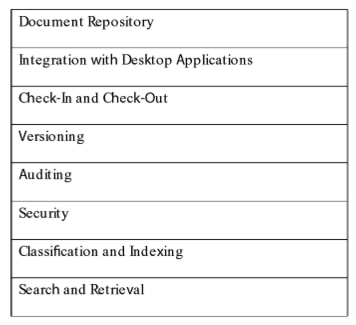
\includegraphics{res/bg-knowledge/edms-components.png}
	\caption{Components of EDMS \citefigure{1_adam_2008}}
	\label{fig:edms-components}
\end{figure}

Later on in the 1990s, \gls{edms} is developed targeting large enterprises with high volume of documents.
It is the improved version of \gls{dip} with workflow functionality.
Workflow functionality enables organizations to passed around scanned document throughout the organization to designated employees.
\gls{edms} also has its own document repository allowing documents to be indexed and tracked using version control.
There are various sub-types of \gls{edms} such as \gls{erms} deals mainly with record keeping.
\gls{ecm} is a suite of applications that manages documents and records.
Now, \gls{edms} acronym is shortened to \gls{dms}.
Figure \ref{fig:edms-components} shows a basic components of \gls{dms}.
Most \gls{dms} applications have these components implemented within.
\begin{description}
	\item[Document Repository] \hfill \\
	Document Repository is a place where indexed documents are stored, usually on a server.
	\item[Integration with desktop applications] \hfill \\
	Allowing user to save documents straight to application after the document is created.
	It is usually a 3rd party add-on embedded in popular office applications such as Microsoft Office.
	\item[Check-in and check-out] \hfill \\
	This feature controls who is allowed to make changes or to read documents.
	Basically, it is a user permission control system.
	\item[Versioning] \hfill \\
	Keeping track of changes by assigning a version number to a document.
	The number is incremented after the document passes major revisions.
	User can access the previous versions of the document.
	\item[Auditing] \hfill \\
	Track who changes document, when, and where.
	Only authorized user can read these information.
	\item[Security] \hfill \\
	Controls how documents should be stored in the server to prevent unauthorized users from attacking the system.
	\item[Classification and indexing] \hfill \\
	Metadata and tags provide more information to documents.
	It helps to search and retrieve documents easier.
	\item[Search and Retrieval] \hfill \\
	Allow user to retrieve documents according to keywords.
	Keywords can be a metadata or contents within a document.
	A system may offer advance search criteria by looking for individual fields and combine with other fields using basic boolean operations (AND, OR, NOT). 
\end{description}

\section{Metadata}
Metadata literally means \enquote{data about data} \cite[p.~1]{baca_2008}.
There is no clear definition on what metadata is because this term is used differently in different communities.
For librarians, it refers to information in the library catalog that help users to find the right book in the library.
For search engines, it means descriptions of web page's contents and keywords used to rank relevant websites.
For others, it refers to a descriptive information of resources in human readable format.
Whatever metadata refers to, they share the following similar usage.
\begin{enumerate}
	\item To identify resources.
	\item To distinguish or bundle similar resources.
	\item To find resources based on search criteria.
\end{enumerate}
There are 3 types of metadata \cite{hodge_2001}.
\begin{description}
	\item[Descriptive metadata] give a description of resources for discovery and identification.
	\item[Structural metadata] describes how component's objects are organized.
	\item[Administrative metadata] indicates information about how resource suppose to be managed.
\end{description}

Electronic documents contain descriptive metadata providing additional information on the document.
The reason for having metadata associate with the document is that they can be indexed in the system.
Index is a systematic arrangement of entries designed to enable users to locate information in a document \cite{def-index}.
User can use metadata to quickly locate documents after they are archived in the system.
The electronic document contains information such as those in figure \ref{metadata-ex-doc}, \ref{metadata-ex-pdf}, and \ref{metadata-ex-png}.
Figure \ref{metadata-ex-doc} shows the metadata of a docx file created by Microsoft Word 2013.
User can edit some metadata fields directly from properties view in Windows 10 or in Microsoft Word.
figure \ref{metadata-ex-png} is the metadata of a \gls{png} file.
It has information on image dimension and bit depth.
User can specify date taken in \enquote{Date taken} field.
\enquote{File} metadata category in figure \ref{metadata-ex-doc} and \ref{metadata-ex-png} are generated automatically by the operating system for every type of file.
The operating system can use this metadata to index the file within the hard disk.
Figure \ref{metadata-ex-pdf} shows metadata in a \gls{pdf} file.
This metadata needs a \gls{pdf} reader software (e.g.\ Adobe Reader, Foxit Reader, etc.) to show it.
Windows 10 can't display this metadata because Windows doesn't have native support for \gls{pdf}.
However, there is a third-party software available\footnote{\url{http://coolsoft.altervista.org/en/pdfpropertyextension}} that displays \gls{pdf}'s metadata on a file explorer.
\begin{figure}[h]
	\centering
	\begin{minipage}{0.45\textwidth}
		\centering
		\includegraphics*[scale=0.6]{res/bg-knowledge/metadata-ex-doc}
	\end{minipage} \hfill
	\begin{minipage}{0.45\textwidth}
		\centering
		\includegraphics*[scale=0.6]{res/bg-knowledge/metadata-ex-doc2}
	\end{minipage} \hfill	
	
	\caption{Microsoft Word Document (docx) metadata viewed Windows 10}
	\label{metadata-ex-doc}
\end{figure}
\begin{figure}[h]
	\centering
	\begin{minipage}{0.45\textwidth}
		\centering
		\includegraphics*[scale=0.6]{res/bg-knowledge/metadata-ex-pdf}
		\caption{\acrfull{pdf} metadata viewed on Adobe Reader DC}
		\label{metadata-ex-pdf}
	\end{minipage} \hfill
	\begin{minipage}{0.45\textwidth}
		\centering
		\includegraphics*[scale=0.6]{res/bg-knowledge/metadata-ex-png}
		\caption{\acrfull{png} metadata viewed on Windows 10}
		\label{metadata-ex-png}
	\end{minipage} \hfill	
\end{figure}

\section{NoSQL}
\gls{nosql} is a database that does not use \gls{sql}.
It refers to any database that does not follow the traditional \gls{rdbms} model.
\gls{sql} is designed to be a query language for relational databases which are usually table-based.
Records are stored in rows and columns represent fields.
On the other hand, \gls{nosql} allows to define fields while creating a record.
Nested values are common in \gls{nosql} databases because \gls{nosql} is aggregate oriented.
Hashes, arrays, and objects can be nested with themselves.

The main characteristic separating \gls{nosql} databases from \gls{rdbms} is that they do not use query languages derived from \gls{sql}. 
The following list shows common features of \gls{nosql} \cite[p.~12-16]{nosql-for-dummies}.
\begin{description}
	\item[Schema agnostic] \hfill \\
	\gls{nosql} databases do not require schema to be defined explicitly.
	Any type of records can be stored without having to know how database stores them internally.
	This improves flexibility when designing document's metadata model.
	Some constraints such as field type and field length do not have to be defined beforehand.
	\gls{nosql} can store mixed data type in the same field.
	If there is a new type of form, we can reuse the native form model by extending it instead of defining a new schema.
	\item[Nonrelational] \hfill \\
	A relational database needs relations to describe how tables relate to each other.
	Unlike \gls{rdbms}, \gls{nosql} databases do not have any relation concept.
	They don not store record's relation.
	Meaning that the metadata model does not have to go through database normalization process to minimize data redundancy.
	Programmer can focus on modelling metadata without having to worry about modelling table relations in \gls{rdbms}.
	
	\item[Highly distributable] \hfill \\
	A single server may not be able to handle all data requests in time.
	Instead of dedicating database on the single server, many servers needed to process queries in parallel.
	Storing data across multiple servers in relational databases is a challenging task.
	\gls{nosql} databases can handle distributed queries as long as connected machines are fast enough to talk to each other.
	\gls{dms} for \gls{ic} needs to be scalable and maintainable.
	Storage space required to store document files and their metadata is expected to grow over time.
	If a single storage server is not enough, \gls{nosql} can use multiple storage servers.
	No need to program new a system to manage distributed queries.
\end{description}

There are many \gls{nosql} storage types available to model the content.
For example, \enquote{Column-oriented database} stores data as columns instead of rows in \gls{rdbms}.
\enquote{Graph store} represents data as nodes and relationships as edges in a graph.
\gls{nosql} databases with \enquote{Document Store} storage type organized data as a hierarchical model with parent-child relationships.
The topmost node in Figure \ref{arch-node} called a root node.
This node represents a record's starting point.
The model must have only one root node.
\gls{dms} for \gls{ic} use \enquote{Document Store} storage type to manage document's metadata.
The reason is that this storage type can query child nodes, not just the parent node.
\begin{figure}[h]
	\centering
	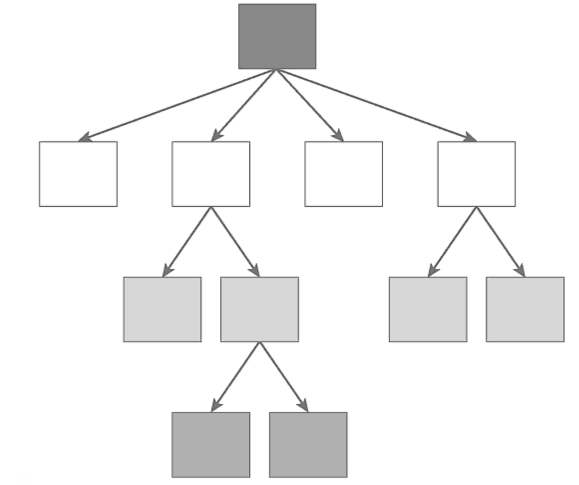
\includegraphics[scale=0.48]{res/bg-knowledge/nosql-hierarchical}
	\caption{The hierarchical organized into a set of parent-child nodes \citefigure{nosql-for-mere-mortals}}
	\label{arch-node}
\end{figure}
Another reason is that programmer can store objects to \gls{nosql} database easily by converting them to \gls{json} objects.

Directed edges connecting between two nodes represents a relationship.
A node where an arrow points called a parent node.
A node where an arrow is pointed called a child node.
The parent node can have many child nodes and each child node can have many parent nodes.

From Figure \ref{metadata-ex-pdf}, a \gls{pdf} metadata can be modelled to hierarchical parent-child relationship as shown in figure \ref{nosql-uml-hiarch-repr}.
Figure \ref{nosql-aggregate-uml} is a data model representation using \gls{uml} notation.
\enquote{PDF} is a root node of the the hierarchical model.
The root node is not necessary for implementation because \enquote{Document Store} had already created it by default.
Thus, the default-created node causes the \enquote{PDF} node to be its child node.
Since the hierarchical model require the root node, it is recommended to have the root node in the model.
Multiplicity constraints indicated by an integer represents maximum allowance number of object instances.
A note symbol (rectangle with right-folded corner) has dotted lines connected to it.
Those lines indicate which metadata are generated automatically by \gls{xmp}.
It restrict user from editing them.
\gls{xmp} is a file labeling technology developed by Adobe Systems Inc..
\gls{xmp} embeds metadata into files during the content creation process \cite{adobe-xml}.
\enquote{Description} and \enquote{Advanced} are \enquote{PDF}'s child nodes.
\enquote{Description} and \enquote{Advanced} also contain their child nodes.
Each node is an object in itself.
\gls{nosql} databases can locate any node within the graph according to any specific queries.
\begin{figure}[ht]
	\centering
	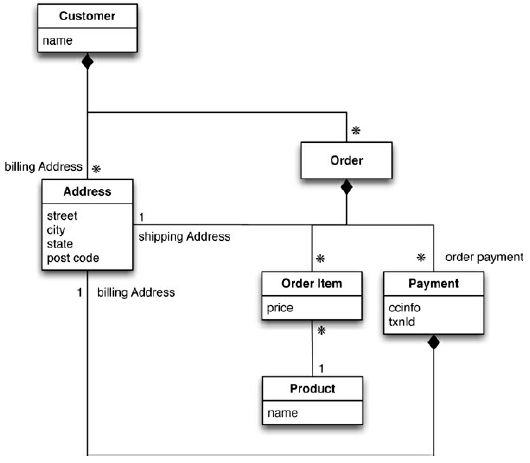
\includegraphics[scale=0.53]{res/bg-knowledge/nosql-nosql-agregate-uml}
	\caption{An aggregate data model in UML notation from figure \ref{metadata-ex-pdf}}
	\label{nosql-aggregate-uml}
\end{figure}
\begin{figure}[ht]
	\centering
	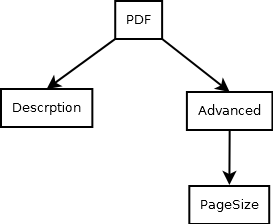
\includegraphics[scale=0.5]{res/bg-knowledge/nosql-uml-hiarch-repr}
	\caption{A hierarchical representation from figure \ref{nosql-aggregate-uml}}
	\label{nosql-uml-hiarch-repr}	
\end{figure}

\begin{normalsize}
\begin{longtable}{C{0.15\textwidth} C{0.15\textwidth} L{0.2\textwidth} L{0.3\textwidth}}
		\caption{Corresponding attributes and fields between figure \ref{nosql-aggregate-uml} and \ref{metadata-ex-pdf}}
		\label{tbl:uml-corespond-pdf} \\
		\hline
		Class & Attribute & Corresponding field in figure \ref{metadata-ex-pdf} & value \\
		\hline
		\endfirsthead
		
		\caption{Corresponding attributes and fields between figure \ref{nosql-aggregate-uml} and \ref{metadata-ex-pdf}} \\
		\hline
		Class & Attribute & Corresponding field in figure \ref{metadata-ex-pdf} & value \\
		\hline
		\endhead
		
		\hline \multicolumn{4}{r}{{Continued on next page}} \\ \hline
		\endfoot
		
		\hline \hline
		\endlastfoot
		
		Description & fileName & File: & dms.pdf \\
		& title & Title: & Document Management System for IC KMITL \\
		& author & Author:  & Apipol Niyomsak \\
		& subject & Subject: & \\
		& dateCreate & Created: & \textbf{1450792574} \\
		& dateModified & Modified: & \textbf{1450792574} \\
		& application & Application: & LaTeX with hyperref package \\
		Keyword & tag & Keywords: & [dms, IC, KMITL]\\
		Advanced & pdfProducer & PDF Producer: & pdfTeX-1.40.16 \\
		& pdfVersion & PDF Version: & 1.5 (Acrobat 6.x) \\
		& location & Location: &  C:\textbackslash Users\textbackslash Apipol\textbackslash Documents\textbackslash \newline 
		TEX\textbackslash dms\_thesis\textbackslash \\
		& fileSizeByte & File Size: & 1909582 \\
		& taggedPDF & Tagged PDF: & \textit{\textbf{false}} \\
		& fastWebView & Fast Web View: & \textit{\textbf{false}} \\
		& totalPage & Number of Pages: & 42 \\
		PageSize & unit & Page Size: & in \\
		& width & Page Size: & 8.50 \\
		& height & Page Size: & 11.00 \\
		\hline
\end{longtable}
\end{normalsize}

Table \ref{tbl:uml-corespond-pdf} summarizes corresponding attributes (figure \ref{nosql-aggregate-uml}) and fields (figure \ref{metadata-ex-pdf}).
Note that bold-highlighted values are stored differently from any other data types.
\enquote{dateCreate} and \enquote{dateModified} have \textit{Date} data type.
When storing date in \gls{nosql}, it converts to UNIX timestamp automatically.
UNIX timestamp (UNIX time, POSIX time, or UNIX epoch) is the number of seconds elapsed since January 1, 1970 (midnight UTC/GMT) \cite{unix-time}.
\enquote{taggedPDF} and \enquote{fastWebView} have \textit{Boolean} data type.
Boolean represents either \textit{true} or \textit{false}.
\gls{nosql} store this data type as a one byte variable.
It use less storage than integer or string to avoid any unexpected side effects of comparison. 
For example, numeric value of \textit{1} is not the same as a boolean value of \textit{true}.
The boolean data type has to perform logical operation with the same data type.
If a programmer would like to store a boolean value, he has to use a boolean data type provided by the programming language.

\enquote{Document store} use \gls{xml}, \gls{json}, \gls{bson}, or \gls{yaml} to manipulate data.
Client have to use REST API provided by the database to query the data.
\gls{rest} is a network-based software architectural style of the World Wide Web \cite{doglio, masse_2012}.
It takes care interactions between client and server.
Client program communicates with the database using \gls{http} through exposed \glspl{api}.

Listing \ref{nosql-uml-json} is a \gls{json} source code implemented from figure \ref{nosql-aggregate-uml}.
\enquote{Document store} databases can import \gls{json} file directly.
Querying from \enquote{Document store} databases will return \gls{json} results.
Some web programming languages such as PHP and Javascript can parse \gls{json} results by converting them to associative arrays.
Thus, programmer can use them to develop their systems.
\begin{normalsize}
\lstinputlisting[style=json, label=nosql-uml-json, caption=\gls{json} source code implementation from figure \ref{nosql-aggregate-uml}]{res/bg-knowledge/nosql-uml-json.json}
\end{normalsize}

\section{Business Process Modelling Notation (BPMN)}
\gls{bpmn} is a graphical notation that depicts the steps in business process \cite{bpmn_omg}.
% What
The goal is to represent business processes using standard graphical notation.
% Who
\gls{bpmn} targets business users and process implementers who need a standard model to communicate their business process.
% Why
Business users create, manage, and monitor processes while process implementers turn processes into a physical implementation. 
\gls{bpmn} does not focus on why, when, and how a process is performed.
But rather what processes, which are the steps to achieve that process, and who should do them.
With \gls{bpmn}, organizations can understand, improve, and control their business processes.
Table \ref{tbl:sum-bpmn-symbol} summarizes \gls{bpmn} symbols that appear in this report along with their descriptions\footnote{Please refer to \url{http://www.omg.org/cgi-bin/doc?formal/11-01-03.pdf} (page 28 - 41) for more details on all available \gls{bpmn} symbols and its detailed descriptions.}.
%TODO UPDATE NEW SYMBOLS AS IT APPEARS IN THIS REPORT
\begin{longtable}{C{0.2\textwidth} L{0.45\textwidth} C{0.3\textwidth}}

	% Setting up header-----------------------------
	
	% First header
	\caption{Summary of \gls{bpmn} symbols \citefigure{bpmn_manual_omg} \cite{bpmn_manual_omg}}
	\label{tbl:sum-bpmn-symbol} \\
	
	\hline
	Element & Description & Notation \\
	\hline
	\endfirsthead
	%----------------------

	% Repeated header
	\caption{Summary of \gls{bpmn} symbols \citefigure{bpmn_manual_omg}} \\
	\hline
	Element & Description & Notation \\
	\hline
	\endhead
	
	\hline \multicolumn{3}{r}{{Continued on next page}} \\ \hline
	\endfoot
	
	\hline \hline
	\endlastfoot
	%----------------------
		
	%-----------------------------------------------
	
	Start Event & 
	Indicates where a process begins &
	\bpmnfig[scale=0.015]{\bpmnSymRepo start-event-none} \\
	
	Intermediate Event &
	Intermediate Event represents a status reached in a process, and it is modelled explicitly.  &
	\bpmnfig[scale=0.02]{\bpmnSymRepo start-event-intermediate} \\
	
	End Event & 
	Indicates where a process ends &
	\bpmnfig[scale=0.015]{\bpmnSymRepo end-event-none} \\
	
	End Event Terminate &
	Terminate all running activities in a process immediately without any error handling. &
	\bpmnfig[scale=0.015]{\bpmnSymRepo end-event-terminate} \\
	
	Message &
	A Message represents information communicating between two participants. &
	See two rows below. \\
	
	Start Message Event &
	An event triggers a process to start when a Message arrives from a participant. &
	\bpmnfig[scale=0.025]{\bpmnSymRepo start-event-message} \\
	
	End Message Event &
	A message received from a participant concludes the end of a process. &
	\bpmnfig[scale=0.025]{\bpmnSymRepo end-event-message} \\
	
	Activity &
	An activity performs work within a business process.
	It can be single or compound.
	It is an executable element of \gls{bpmn}. &
	See three rows below. \\
	
	Task & 
	A Task is a unit of work performs in a process.
	It has a task name inside a rounded rectangle notation.
	The task is used when process can not be broken down any further.
	It has no internal parts, representing a single action. &
	\bpmnfig[scale=0.03]{\bpmnSymRepo task} \\	
	
	User Task &
	A subtype of Task in which human is the one who perform a task with the help of a software application. &
	\bpmnfig[scale=0.035]{\bpmnSymRepo user-task} \\	
	
	Sub-Process &
	A Sub-Process composes of a single activity or compound activity.
	It refers to a process that can be broken down to a finer detail.
	The collapsed Sub-Process hides activity details from the diagram indicated by a plus sign.
	The expanded one shows activities inside the diagram indicated by a minus sign. &
	\bpmnfig[scale=0.03]{\bpmnSymRepo subprocess-collapsed}
	Collapsed Sub-Process
	\bpmnfig[scale=0.03]{\bpmnSymRepo subprocess-expanded}
	Expanded Sub-Process \\	
	
	Activity Looping &
	Activity Looping loops itself continuously until its boolean condition becomes \textit{true}.
	It evaluates condition every time before/after it performed for every loop iteration. &
	\bpmnfig[scale=0.04]{\bpmnSymRepo task-loop} \\	
		
	Normal Flow &
	Shows activity order performed in a process &
	\bpmnfig[scale=0.02, angle=-45]{\bpmnSymRepo connection} \\
	
	Conditional Flow &
	It will perform the outgoing sequence flow if and only if conditional expression evaluates to \textit{true}. &
	\bpmnfig[scale=0.02, angle=-45]{\bpmnSymRepo conditional-flow} \\

	Default Flow &
	Execute this flow if all other outgoing conditional expression evaluate to \textit{false}. &
	\bpmnfig[scale=0.02, angle=-45]{\bpmnSymRepo default-flow} \\

	Message Flow &
	Indicates a Message sent between two participants. &
	\bpmnfig[scale=0.025, angle=-45]{\bpmnSymRepo message-flow} \\

	Gateway & 
	Controls branching, merging, forking, and joining multiple sequence flow paths. 
	& See four rows below. \\
	
	Exclusive Gateway &
	Creates multiple alternative paths in a process.
	If one of the conditional expression evaluates to \textit{true}, it executes that path without evaluating others.
	It has the same functionality as conditional flow.
	The difference is that Exclusive Gateway allows multiple branching from the same node. &
	
	\begin{center}
	\begin{minipage}{0.1\textwidth}
		\bpmnfig[scale=0.025]{\bpmnSymRepo gateway-none}
	\end{minipage}
	or
	\begin{minipage}{0.1\textwidth}
		\bpmnfig[scale=0.025]{\bpmnSymRepo gateway-xor}
	\end{minipage}
	\end{center} \\
	
	Event-based Gateway &
	Evaluates which event occurs first, not which condition is met.
	If that event occurred, go to that outgoing flow and discard other conditions. &
	\bpmnfig[scale=0.025]{\bpmnSymRepo gateway-eventbased} \\
	
	Parallel Gateway &
	Parallel gateway is used to create and to combine parallel flows.
	It represents multiple concurrent activities performing at the same time.
	It doesn't evaluate any condition or event before execution.
	Parallel gateway will wait for all incoming flows to finish before proceeding to the next outgoing flow. &
	\bpmnfig[scale=0.025]{\bpmnSymRepo gateway-parallel} \\	
	
	Inclusive Gateway &
	Evaluates all conditional expression unlike the exclusive gateway.
	It is used to create alternative parallel paths.
	If there are multiple conditional expressions evaluated to \textit{true}, those flows will be executed independently in parallel. &
	\bpmnfig[scale=0.025]{\bpmnSymRepo gateway-or} \\		
	
	Data Object &
	Provide information about what activity requires to perform and/or what they produce. 
	Data Object can also refer to a collection of Data Objects.
	Data Input have a white arrow on the top corner.
	It is placed before activity starts indicating what that activity requires.
	Data Output have a shaded arrow on the the corner.
	It is placed after activity finished indicating what activity produces. &
	\bpmnfig[scale=0.025]{\bpmnSymRepo data-object}
	Data Object
	\bpmnfig[scale=0.025]{\bpmnSymRepo data-input}
	Data Input
	\bpmnfig[scale=0.025]{\bpmnSymRepo data-output}
	Data Output \\
	
	Text Annotation &
	Text Annotation provides additional information to a \gls{bpmn} diagram reader.
	Its notation composes of a opening square bracket with a dashed line attached on the left.
	The dashed line can connect to any \gls{bpmn} element.
	The bracket contains a descriptive text on the right.
	It scales vertically to cover multiple lines of text.
	&
	\bpmnfig[scale=0.025]{\bpmnSymRepo text-annotation} \\
	
	Pool &
	A Pool represents a collaboration between participants in a process.
	It can be partitioned to multiple smaller Pools called Lane.
	Each Lane assigns to one participant.
	The Participant is a person, machine, group of persons or machines responsible for the process execution within the Pool.
	The Pool is a container of activities.
	All activities inside the Pool can cross boundaries to any Lane but not outside the Pool.
	There are two types of Pool---horizontal and vertical.
	Both of them has the same functionality.
	The difference is their alignment.
	A horizontal one expands horizontally while a vertical one expands vertically.
	
	&
	\bpmnfig[scale=0.03]{\bpmnSymRepo participant}
	Horizontal Pool
	\bpmnfig[scale=0.03]{\bpmnSymRepo collaboration}
	Horizontal Pool with Lanes
	\bpmnfig[scale=0.03, angle=-90]{\bpmnSymRepo participant}
	Vertical Pool
	\bpmnfig[scale=0.03, angle=-90]{\bpmnSymRepo collaboration}
	Vertical Pool with Lanes. \\
	
	\hline

\end{longtable}

\newpage

% Teach readers how to read a BPMN diagram by example.
\begin{figure}[t]
	\centering
	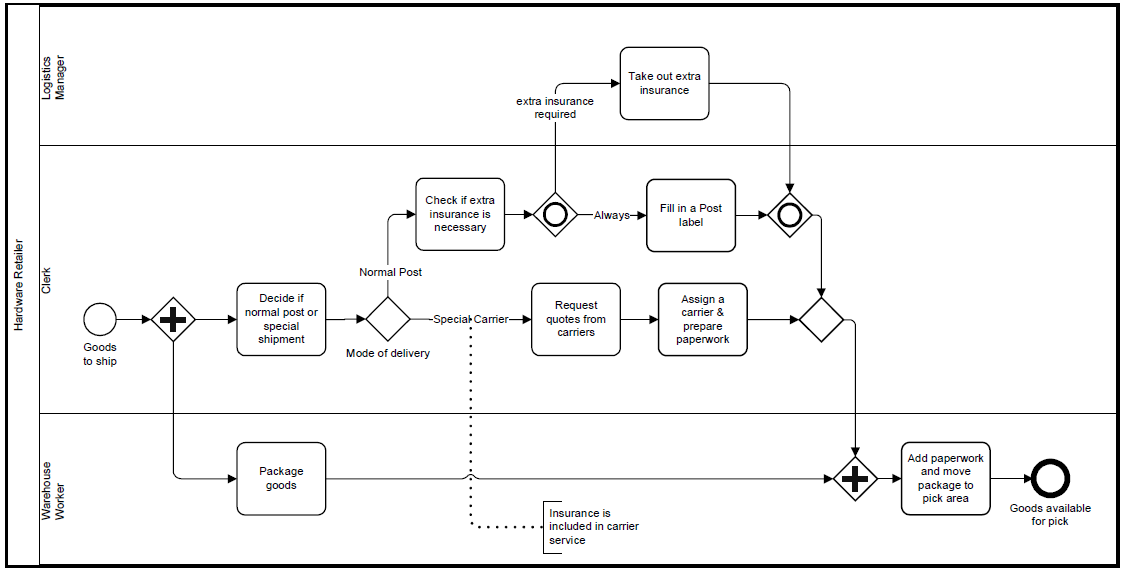
\includegraphics[scale=0.55]{res/bg-knowledge/bpmn-example}
	\caption{Shipment Process of a hardware retailer \citefigure{bpmn_manual_example_omg} \cite{bpmn_manual_example_omg}.}
	\label{fig:bpmn-example}
\end{figure}

Figure \ref{fig:bpmn-example} provides an example of a \gls{bpmn} diagram.
Note that all gateways come in pairs.
Exclusive Gateway have to indicate where branching starts and merges.
Parallel Gateway and Inclusive Gateway need to synchronize flows because branched tasks are performed in parallel.
Synchronization is to ensure that all branched tasks are completed before going to the next flow.

The figure shows steps of hardware retailer's shipment process of shipping goods to customers.
There are three participants involved in the hardware retailer---a warehouse worker, a clerk, and a logistics manager.
A Start Event (\includegraphics[scale=0.0035]{\bpmnSymRepo start-event-none}) marks the beginning of a process.
An End Event (\includegraphics[scale=0.0035]{\bpmnSymRepo end-event-none}) marks the end of the process.
Arrows navigates the flow to each node in the diagram.

\enquote{Goods to ship} is a trigger of a process.
A Parallel Gateway (\includegraphics[scale=0.005]{\bpmnSymRepo gateway-parallel}) with outgoing two flows indicates that task \enquote{Decide if normal post or speical shipment} and \enquote{Package goods} have to be done in parallel.
While clerk is deciding if goods is a normal postal or special shipment, the warehouse worker can start packaging the goods.
Next clerk's task is to decide a \enquote{Mode of delivery} indicated by an Exclusive Gateway (\includegraphics[scale=0.005]{\bpmnSymRepo gateway-none}).
The gateway is not responsible for clerk's decision, but rather the task before it.
If the clerk decides that goods are a special carrier, the clerk will perform \enquote{Request quotes from carriers} and \enquote{Assign a carrier \& prepare paperwork} task.
A special carrier includes a carrier service denoted by a Text Annotation (\includegraphics[scale=0.005]{\bpmnSymRepo text-annotation}).
If the clerk decides that goods are normal post, the clerk will perform \enquote{Check if extra insurance is necessary} task.
While the clerk is filling in a post label, if goods requires an extra insurance, the logistics manager will take out extra insurance.
An Inclusive Gateway (\includegraphics[scale=0.005]{\bpmnSymRepo gateway-or}) ensures that logistic manager will deal with goods if they need the extra insurance.
Finally, the warehouse worker will add paperwork and move package to a pick area.
All goods are ready to ship to customers.